\documentclass[a4paper,12pt]{article}

\usepackage[margin=1.5cm]{geometry}
\usepackage[T1]{fontenc}
\usepackage{lmodern}
\usepackage{tikz}
\usetikzlibrary{arrows.meta,calc,fit}

\pagestyle{empty}

\begin{document}

\begin{center}
    {\Large\bfseries System Architecture}\\[4pt]
    {\large Leave Management System}
\end{center}

\vspace{0.3cm}

\begin{center}
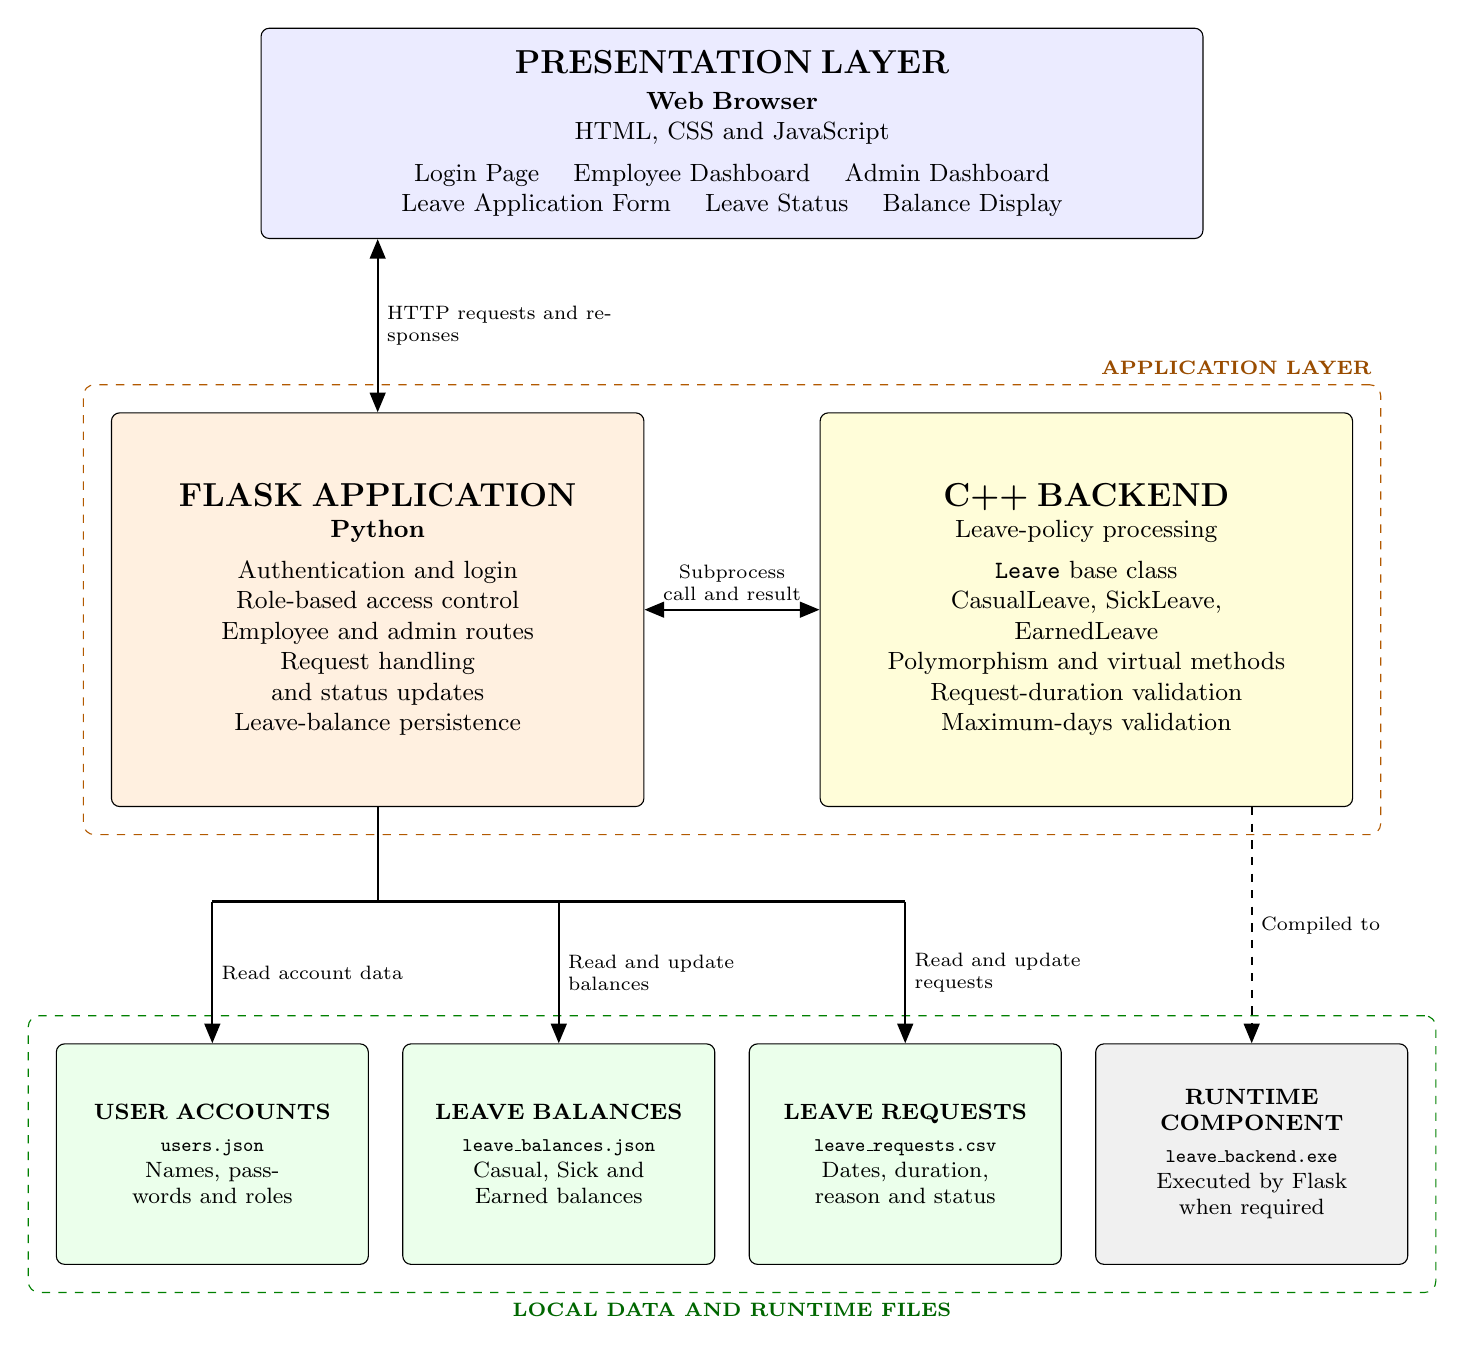
\begin{tikzpicture}[
    layer/.style={draw, rounded corners=3pt, align=center,
                  inner sep=8pt, font=\small},
    datanode/.style={layer, font=\footnotesize, fill=green!8,
                     text width=3.4cm, minimum height=2.8cm},
    lbl/.style={font=\scriptsize, align=left, inner sep=1pt},
    flow/.style={thick, -{Triangle[length=2.5mm,width=2mm]}},
    flow2/.style={thick, {Triangle[length=2.5mm,width=2mm]}-{Triangle[length=2.5mm,width=2mm]}},
    container/.style={dashed, rounded corners=4pt, inner sep=0.35cm}
]

% --------------------------------------------------
% PRESENTATION LAYER
% --------------------------------------------------
\node[layer, anchor=north, fill=blue!8, text width=11.4cm]
    (browser) at (0,0) {
    \textbf{\large PRESENTATION LAYER}\\[2pt]
    \textbf{Web Browser}\\
    HTML, CSS and JavaScript\\[4pt]
    Login Page \quad Employee Dashboard \quad Admin Dashboard\\
    Leave Application Form \quad Leave Status \quad Balance Display
};

% --------------------------------------------------
% APPLICATION LAYER
% --------------------------------------------------
\node[layer, anchor=north, fill=orange!12, text width=6.2cm, minimum height=5cm]
    (flask) at ($(browser.south)+(-4.5,-2.2)$) {
    \textbf{\large FLASK APPLICATION}\\
    \textbf{Python}\\[4pt]
    Authentication and login\\
    Role-based access control\\
    Employee and admin routes\\
    Request handling\\and status updates\\
    Leave-balance persistence
};

\node[layer, anchor=north, fill=yellow!15, text width=6.2cm, minimum height=5cm]
    (cpp) at ($(browser.south)+(4.5,-2.2)$) {
    \textbf{\large C++ BACKEND}\\
    Leave-policy processing\\[4pt]
    \texttt{Leave} base class\\
    CasualLeave, SickLeave,\\EarnedLeave\\
    Polymorphism and virtual methods\\
    Request-duration validation\\
    Maximum-days validation
};

% --------------------------------------------------
% DATA AND RUNTIME ROW
% --------------------------------------------------
\coordinate (bus) at ($(browser.south |- flask.south)+(0,-1.2)$);
\coordinate (row) at ($(browser.south |- flask.south)+(0,-3.0)$);

\node[datanode, anchor=north] (users) at ($(row)+(-6.6,0)$) {
    \textbf{USER ACCOUNTS}\\[2pt]
    {\scriptsize\texttt{users.json}}\\
    Names, passwords and roles
};

\node[datanode, anchor=north] (balances) at ($(row)+(-2.2,0)$) {
    \textbf{LEAVE BALANCES}\\[2pt]
    {\scriptsize\texttt{leave\_balances.json}}\\
    Casual, Sick and Earned balances
};

\node[datanode, anchor=north] (requests) at ($(row)+(2.2,0)$) {
    \textbf{LEAVE REQUESTS}\\[2pt]
    {\scriptsize\texttt{leave\_requests.csv}}\\
    Dates, duration, reason and status
};

\node[datanode, anchor=north, fill=gray!12] (exe) at ($(row)+(6.6,0)$) {
    \textbf{RUNTIME COMPONENT}\\[2pt]
    {\scriptsize\texttt{leave\_backend.exe}}\\
    Executed by Flask when required
};

% --------------------------------------------------
% DASHED CONTAINERS (outline only, drawn after the boxes)
% --------------------------------------------------
\node[container, draw=orange!70!black, fit=(flask)(cpp)] (appbox) {};
\node[container, draw=green!50!black, fit=(users)(balances)(requests)(exe)] (databox) {};

\node[anchor=south east, font=\scriptsize\bfseries, text=orange!60!black]
    at (appbox.north east) {APPLICATION LAYER};
\node[anchor=north, font=\scriptsize\bfseries, text=green!40!black]
    at (databox.south) {LOCAL DATA AND RUNTIME FILES};

% --------------------------------------------------
% CONNECTORS
% --------------------------------------------------
% Browser <-> Flask
\draw[flow2] (browser.south -| flask.north) -- (flask.north)
    node[midway, right=2pt, lbl, text width=3.2cm] {HTTP requests and responses};

% Flask <-> C++ backend
\draw[flow2] (flask.east) -- (cpp.west)
    node[midway, above=2pt, lbl, align=center, text width=2.1cm]
    {Subprocess call and result};

% Flask -> data files (shared bus, vertical drops)
\draw[thick] (flask.south) -- (flask.south |- bus);
\draw[thick] (users.north |- bus) -- (requests.north |- bus);

\draw[flow] (users.north |- bus) -- (users.north)
    node[midway, right=2pt, lbl, text width=2.5cm] {Read account data};
\draw[flow] (balances.north |- bus) -- (balances.north)
    node[midway, right=2pt, lbl, text width=2.5cm] {Read and update balances};
\draw[flow] (requests.north |- bus) -- (requests.north)
    node[midway, right=2pt, lbl, text width=2.5cm] {Read and update requests};

% C++ backend -> compiled executable
\draw[flow, dashed] (exe.north |- cpp.south) -- (exe.north)
    node[midway, right=2pt, lbl] {Compiled to};

\end{tikzpicture}
\end{center}

\end{document}